\documentclass[10pt,twoside,twocolumn,openany]{book}
\usepackage[bg-letter]{dnd} % Options: bg-a4, bg-letter, bg-full, bg-print, bg-none.
\usepackage[english]{babel}
\usepackage[utf8]{inputenc}
\usepackage{graphicx}


% Start document
\begin{document}
\fontfamily{ppl}\selectfont % Set text font

\chapter{Races}

% Lionfolk race
\section{Lionfolk}

One of the beastfolk races to emigrate from Krata over three millenia ago, lionfolk were the first beastfolk to achieve acknowledgement, if not acceptance. Honorable and faithful, sometimes to a fault, lionfolk espouse valor and virtue, traits that endeared themselves to some of the nine clans, especially the White Lance. In Beast Speech, lionfolk are called the nevayuu, meaning "we who fight".

\subsection{Broad and Mighty}

Lionfolk are big and well-muscled, standing well over 6 feet tall, sometimes even reaching 7 feet. Lionfolk, like the rest of the beastfolk, have small claws for nails, though they are usually not sharp enough for combat. Lion have blond, bushy hair on their forearms and shins, and they generally have light skin tones, but they show only mild effects of prolonged exposure to sunlight over long periods. Male lionfolk have bushy blond hair and beards that resemble a lion's mane, but can sometimes be reddish in hue. Lionfolk, like all beastfolk, walk on human shaped feet instead of animal-like paws. Lionfolk faces resemble that of a lion, with eyes that vary in color like that of a human.\\
Lionfolk show little preference in the clothing they wear, emulating the fashion of the province they live in, though it is more to keep up appearances as most clothes sold in Korrik don't fit lionfolk easily. Most lionfolk prefer to wear shirts and pants instead of the overly ostentatious clothes many of the wealthy in the island nation put on.\\
Due to their strong affiliation with the White Lance, lionfolk are found primarily in Whiteguard, though pockets will be spotted throughout the country's major cities.

\subsection{Proud and Honorable}

Lionfolk live by strong ethical and moral codes, placing the needs and lives of others over their own. Though their adherence to their ways can make them rigid and arrogant, they are, at best, honest and forthright. This demeanor stems from a culture they adopted while living on Krata. They placed loyalty to their leaders and perfection of skill above all else. In time, this created a society of warriors who valued honor, courage, and might in battle above all else. This has bled into their identity today.\\
The ethical and moral norms lionfolk place on themselves can vary between each lionfolk; no two are the same. However, their interpretation of any norm, no matter how few or minor, is strict, maybe even rigid. 
\begin{center}
	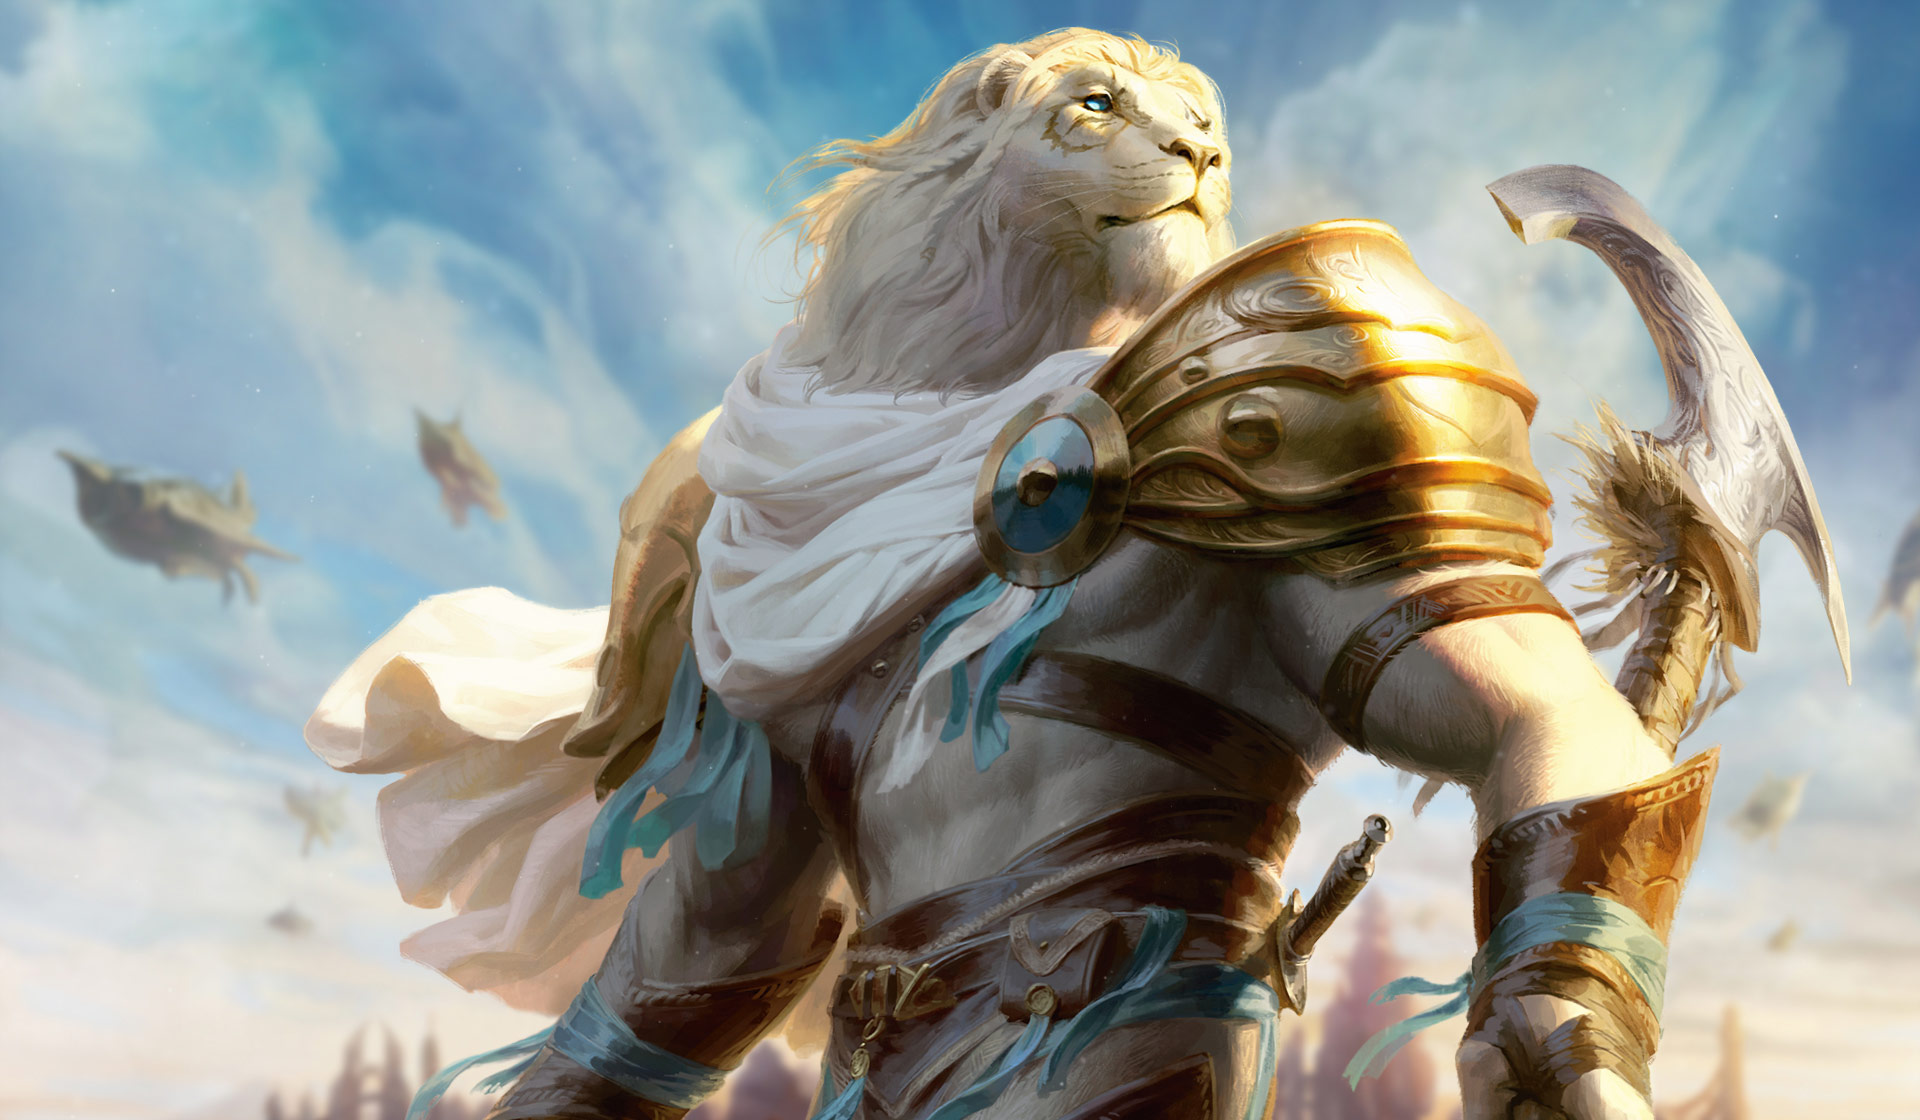
\includegraphics[width=90mm,scale=0.5]{img/lionfolk.jpg}
\end{center}
In most cases, lionfolk will adopt the rules of their job or career, holding to all rules with almost ironclad devotion. This can create a penchant for fanaticism, or even an inflexible interpretation of the law. From a moral perspective, they will often hold to certain acts as incongruous to their ways or opposite to what they believe, they will avoid it completely, even going so far as to report those who commit even a minor offense.

\subsection{The Cause is Everything}

To lionfolk, they must have a strong reason to embark on a great adventure in an unknown land. Most often, lionfolk try to embrace a cause they will devote themselves to for the rest of their lives. It could be something as simple as fighting evil where they find it or exterminate a threat to their family, but is always derived from the rules and norms they follow. A cause that would force a lionfolk to leave home will inevitably draw them to an adventuring life, but they will have difficulty getting past the fact many do not share their frame of mind, especially in lawless lands where rules mean nothing. Spreading law to such lands might be such a reason, however.

\subsection{Lionfolk Names}

Lionfolk, like all beastfolk, adopt traditionally human names, but will also take names derived from characteristics of beasts.\\
\textbf{Male:} Any human name, as well as Claw, Tooth, Leo, or Mane\\
\textbf{Female:} Any human name, as well as Paw and Fur\\

\subsection{Lionfolk Traits}

Your lionfolk character has a number of traits in common with all other lionfolk, many of which involve either might or mind.You are part of A proud and honorable race that embraces a cause or oath for life. \\
\indent \textbf{Ability Score Increase.} Your Strength score increases by 2.\\
\indent \textbf{Age.} Lionfolk consider themselves adults at age 33. They commonly live about 300 years, but some have lived as long as 325 years, despite those lionfolk being markedly infirm by that time. \\
\indent \textbf{Alignment.} Lionfolk value order and honor above all things, tending towards law. Lionfolk have a strong disposition towards good, but when pushed to follow the rules or follow their heart, many will choose the former.\\
\indent \textbf{Size.}  Lionfolk are tall and muscular, standing between 6'2” and 7'2” when they reach adulthood. They usually weigh around 200–270 lbs. Your size is Medium.\\
\indent \textbf{Speed.} Your base walking speed is 30 feet.\\
\indent \textbf{Brave.} You have advantage on saving throws against being frightened.\\
\indent \textbf{On the Prowl.} You have advantage on Wisdom (Perception) checks that rely on hearing or smell.
\indent \textbf{Languages.} You can speak, read, and write Common and Beast Speech. Beast Speech is a language exclusive to beastfolk, derived from their own need for cultural identity and privacy. Beast Speech is simple, emphasizing many words involving the letter n, and words can have multiple, but similar, meanings, so it is a language where misinterpretation can easily occur.\\
\indent \textbf{Subrace.} Two main subraces of Lionfolk live in this world: Ironfang and Whitemane. Choose one of these subraces.

\subsubsection{Ironfang}

Ironfang lionfolk are aggresive and passionate regarding their goals. They believe that only by being tested that their kind will be able grow. Dominance, strength, and valor are the best qualities a good Ironfang will have. \\
Ironfang are natural soldiers and commanders and believe that war is the gear that moves society and enable the lionfolk to become stronger.\\
\indent \textbf{Ability Score Increase.} Your Intelligence score increases by 1.\\
\indent \textbf{Bite.} You have no trouble fighting with everything you have available. You are now proficient with your unarmed strikes, that dea 1d6 damage plus your Strength modifier.\\
\indent \textbf{Survivalist.} You have proficiency in the Survival skill.
\subsubsection{Whitemane}
Whitemane lionfolk are kind and have a strong sense of freedom. Whitemanes tend to look before they leap, and always have a plan of action. Unlike the Ironfang, they have no trouble interacting with other members of this world and are always ready to cooperate. Whitemanes are present in any kind of position in a social hierarchy, from a political advisor to a street merchant.\\
\indent \textbf{Ability Score Increase.} Your Charisma score increases by 1.\\
\indent \textbf{Lion Tactics.} Allies within 5 feet of you do not provoke opportunity attacks so long as they remain within 5 feet of you while moving.\\
\indent \textbf{Natural Leader.} You have proficiency in the Persuasion skill.

\newpage

% Ksanir race
\section{Ksanir}

Banished from Krata millenias ago, Ksanir are considered to be the most dangerous of the beastfolk races. Unpredictable and calculating, the Ksanir value the dark arts and subtlety. Unlike most adventurers who seek gold and glory, this panther-like race prefers to seek knowledge and enlightenment. In Beast Speech, the Ksanir are called the ketalvu, which means "we who lurk in the shadows". 

\subsection{Slender and Obscure}

Ksanir are tall, thing, and quick. They stand well over 6 feet tall, but rarely reach more than 7 feet. They have panther-like features, such as dark skin tones, thin dark hair over their whole body, and sharp claws for combat. Their eyes tend to be yellow or green, but from time to time, it is possible to spot a Ksanir with dark red or even cold light blue eyes.\\
Ksanir tend to wear light and elastic clothing, so as to not slow down their movement. Those clothes rarely emulate the fashion from the place they live in, tending to be of darker color and more tribal, usually in shades of dark green, blue, and mostly black.

\subsection{Sly and Cautious}

Ksanir live by very weak moral and ethical codes, usually placing their needs above the needs of others, including their own kind. They have no loyalties, no true friends, for all others are mere sheep. The true enemies of the Ksanir, are those who are smart and brave enough not to be manipulated by their tactics.
Ksanir do their best to blend in with the crowd, and prove themselves worthy until the almost very end, when they usually play their ultimate card, and reap their unjust reward. 
\begin{center}
	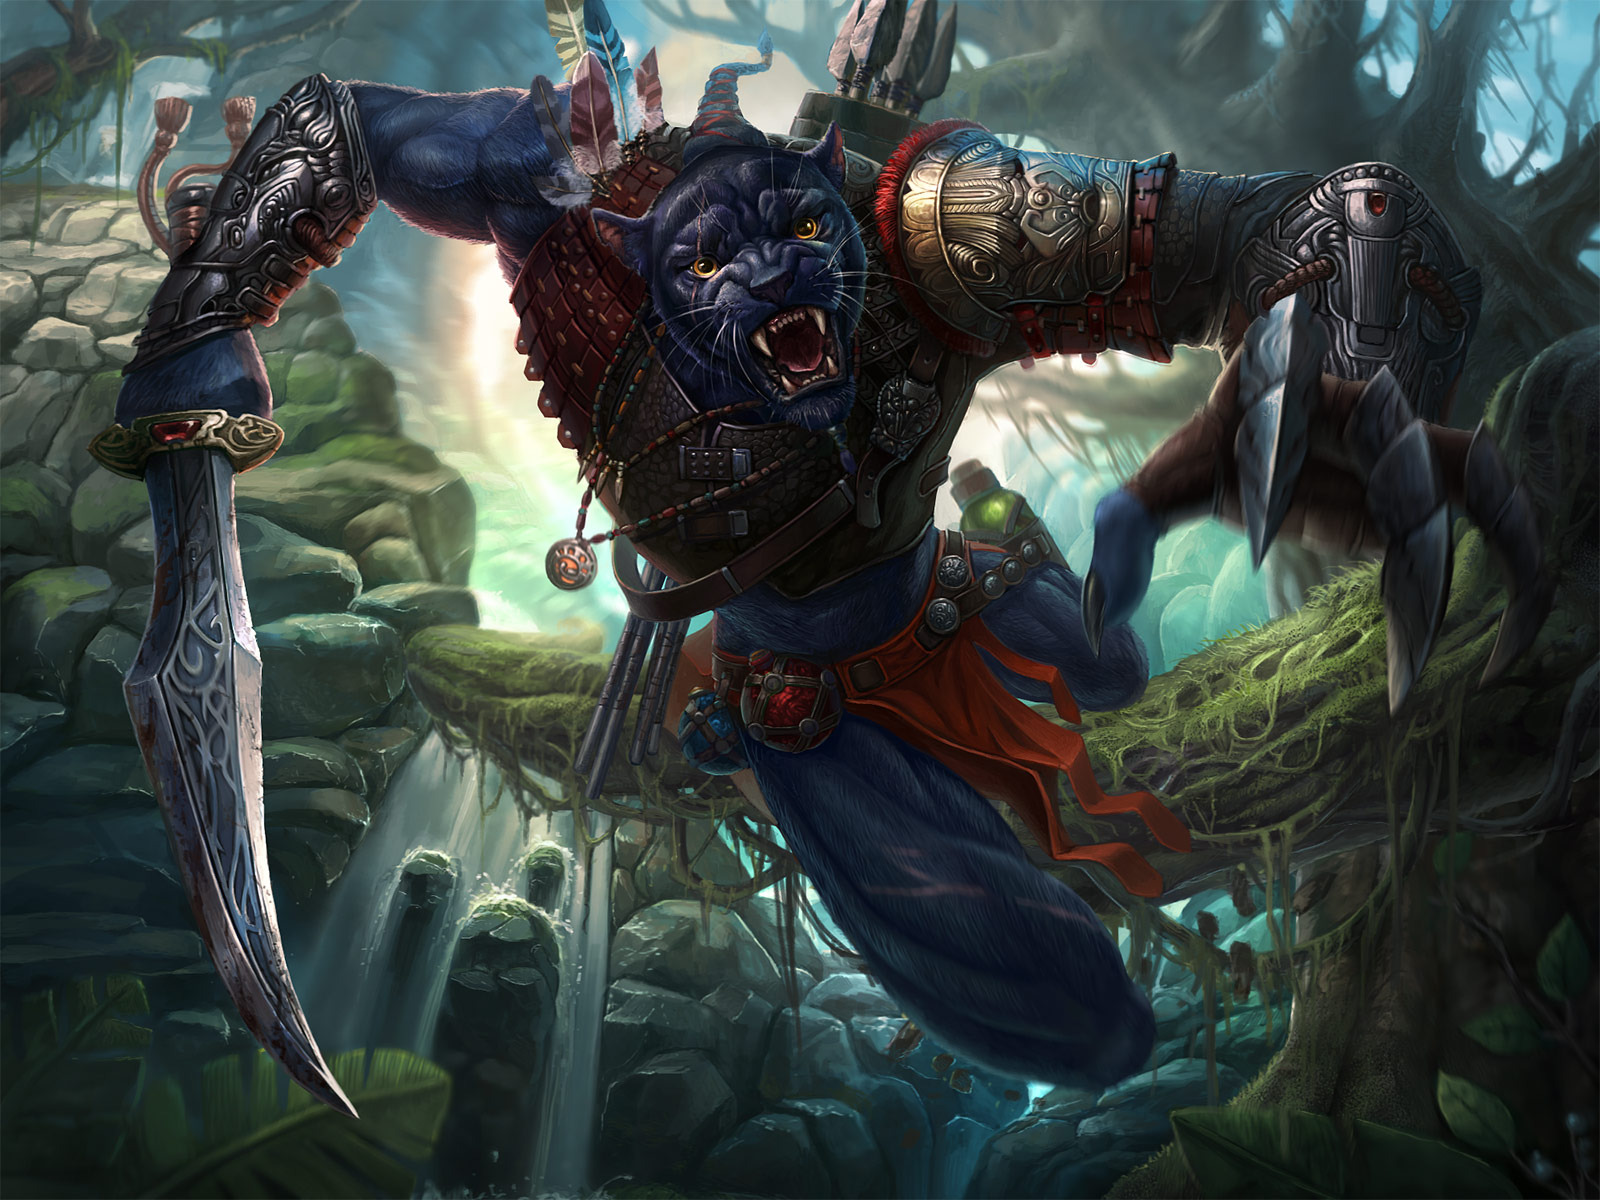
\includegraphics[width=90mm,scale=0.5]{img/ksanir.jpg}
\end{center}
\newpage
Moreover, they are taught to fend for themselves and crave for their desires since they are very young, Ksanir tend to have a very difficult upbringing. Since having a family is not one of the values shared by the Ksanir race, children are sometimes abandoned or sold as slaves. They learn quickly to trust no one, not even their own parents or what they thought were friends. Due to these reasons, members of the Ksanir race are few. \\

\subsection{Hungry for Knowledge}

Ksanir are often driven by knowledge of the dark arts or forbidden knowledge. For a Ksanir to embark on a quest on a land unknown to him, there must be a rumor or a promise of empowering himself with knowledge of the unknown. Ksanir usually don't share knowledge, not even amongst themselves, for they find it to be the greatest of treasures, and by sharing it, all that was acquired becomes a simple commodity.\\
Ksanir will usually kill or do other acts that will usually end up in strong punishment for their actions. No matter the difficulty, they believe in the end that if the way is lit, that means the path was cleared; therefore, there is no reward for the task.

\subsection{Ksanir Names}

Ksanir often choose their names based on their perceived traits or their first accomplishment on life; therefore, there is usually no distinction between male or female names. Also, since they don't honor the tradition of family and its associated values, Ksanir don't have family names.\\
Ksanir usually incorporate a persona when interacting with others so as not to reveal their true name and nature.\\
\textbf{Names:} Vicious, Cunning, Swift, Ravenous, Sly, Mischief, Guile, Tyrant, Sage.

\subsection{Ksanir Traits}
Ksanir traits reflect their harsh life and their desire to become stronger through the possession of knowledge that they know or are willing to learn how to use. \\
\indent \textbf{Ability Score Increase.} Your Intelligence score increases by 2, and your Dexterity score increases by 1.\\
\indent \textbf{Age.} Ksanir consider themselves adults at age 26. It is speculated that they are able to live up to t 130 years, but there are no known reports of a Ksanir surviving that long. \\
\indent \textbf{Alignment.} Ksanir value survival and knowledge above all things, tending towards a chaotic behavior. Their actions usually have evil or even a neutral intent, as long as it doesn't interfere with their goals.\\
\indent \textbf{Size.}  Ksanir are slender and tall, standing between 6.0” and 7.0” when they reach adulthood. They usually weigh around 150–220 lbs. Your size is Medium.\\
\indent \textbf{Speed.} Your base walking speed is 30 feet.\\
\indent \textbf{Darkvision.} Used to fending yourself off in the dark, you have superior vision under dark and dim conditions. You can see in dim light within 60 feet of you as if it were bright light, and in darkness as if it were dim light. You can’t discern color in darkness, only shades of gray. \\
\indent \textbf{On the Prowl.} You have advantage on Wisdom (Perception) checks that rely on hearing or smell.\\
\indent \textbf{No Stone Unturned.} You are able to use your claws so as to have the same outcome of using Thieves' Tools. You are proficient while using them.\\
\indent \textbf{Manipulative.} You have proficiency in the Deception skill.\\
\indent \textbf{Illusory Distraction.} You know the \textit{Minor Illusion} cantrip. When you reach 3rd level, you can cast the \textit{Disguise Self} spell once per day or after you take a long rest, whichever comes first, without using a spell slot. Intelligence is your spellcasting ability for both these spells.\\
\indent \textbf{Languages.} You can speak, read, and write Common, one standard language of your choice and Beast Speech. Beast Speech is a language exclusive to beastfolk, derived from their own need for cultural identity and privacy. Beast Speech is simple, emphasizing many words involving the letter n, and words can have multiple, but similar, meanings, so it is a language where misinterpretation can easily occur.\\
% End document
\end{document}
